\addcontentsline{toc}{chapter}{Appendices}

% The \appendix command resets the chapter counter, and changes the chapter numbering scheme to capital letters.
%\chapter{Appendices}
\appendix
\chapter{Datasets used}
\label{appendixlabel1}

This appendix described the different datasets used in analyses performed in this thesis. It includes datasets of both modern and ancient genomes 

\section{Antonio et al 2019}

Samples from Antonio et al (2019)\cite{antonio2019ancient}. Looking at the population genomics of ancient Rome. 

This dataset consists of 134 shotgun-sequenced individuals from 12,000 years ago to the present day. Coverage ranges from 0.4x - 4x (median 1.05x). 

Aligned reads in .bam format were downloaded from the ENA under accession number PRJEB32566.

\section{Margaryan et al 2020}

Samples from Margaryan et al 2020 \cite{margaryan2020population}, looking at the population genomics of Vikings.  

This dataset consists of 442 shotgun-sequenced individuals from the Bronze Age to Medieval and Early Modern ages. Mean coverage of ~1x. X individuals did not have enough data to estimate recalibration parameters and were excluded from the rest of the analysis.

Aligned reads in .bam format were downloaded from the ENA under accression number PRJEB37976. 

\section{Rivollat et al 2020}

Samples from Rivollat et al (2020)\cite{rivollat2020france}. Looking at the population genomics of France and Germany. 

This dataset consists of 101 captured individuals from 7000–3000 BCE. years ago to the present day. 

Aligned reads in .bam format were downloaded from the ENA under accession number PRJEB36208.


\section{Brunel et al 2018}

Samples from Brunel et al (2018)\cite{Brunel12791}. Looking at the population genomics of France. 

This dataset consists of 52 shotgun sequenced individuals from Mesolithic to the Iron Age. 

Aligned reads in .bam format were downloaded from the ENA under accession number PRJEB36208.

\section{Allentoft et al 2015}

Samples from Allentoft et al 2015 \cite{Allentoft2015}. Looking at the population genomics Bronze Age Eurasia. 

This dataset consists of 20 shotgun sequenced individuals. 

Aligned reads in .bam format were downloaded from the ENA under accession number PRJEB9021.

\section{Broushaki et al 2016}

Samples from Broushaki et al 2016 \cite{Broushaki2016b}. Looking at the population genomics Bronze Age Eurasia. 

This dataset consists of 1 shotgun sequenced individual.

Aligned reads in .bam format were downloaded from the ENA under accession number xxxx.

\section{Cassidy et al 2016}

Samples from Cassidy et al 2016 \cite{Cassidy368}. Looking at the population genomics of the Neolithic and Bronze Age migrations to Ireland. 

This dataset consists of 4 shotgun sequenced individuals.

Aligned reads in .bam format were downloaded from the ENA under accession number PRJEB11995.

\section{de Barros Damgaard et al 2018a}

The first horse herders and the impact of early Bronze Age steppe expansions into Asia.

Samples from de Barros Damgaard et al 2018a \cite{deBarrosDamgaardeaar7711}.

This dataset consists of 34 shotgun sequenced individuals.

Aligned reads in .bam format were downloaded from the ENA under accession number PRJEB26349.

\section{de Barros Damgaard et al 2018b}

137 ancient human genomes from across the Eurasian steppes

Samples from de Barros Damgaard et al 2018b \cite{de2018137}.

This dataset consists of 58 shotgun sequenced individuals.

Aligned reads in .bam format were downloaded from the ENA under accession number PRJEB20658.

\section{Gamba et al 2014}

Genome flux and stasis in a five millennium transect of European prehistory

Samples from  Gamba et al 2014 \cite{Gamba2014}.

This dataset consists of 10 shotgun sequenced individuals.

Aligned reads in .bam format were downloaded from the Sequence Read Archive (SRA) under the accession code SRP039766.

\section{Gunther et al 2015}

Genomic diversity and admixture differs for Stone-Age Scandinavian foragers and farmers

Samples from Gunther et al 2015 \cite{gunther2015ancient}.

This dataset consists of 2 shotgun sequenced individuals.

Aligned reads in .bam format were downloaded from the ENA under accession number PRJEB9783.

\section{Hofmanová et al 2016}

Early farmers from across Europe directly descended from Neolithic Aegeans

Samples from  Hofmanová et al 2016 \cite{Hofmanova2016}.

This dataset consists of 5 shotgun sequenced individuals.

Aligned reads in .bam format were downloaded from the ENA under accession number PRJEB11848.

\section{Jones et al 2015}

Upper Palaeolithic genomes reveal deep roots of modern Eurasians

Samples from  Jones et al 2015 \cite{Jones2015}.

This dataset consists of 2 shotgun sequenced individuals.

Aligned reads in .bam format were downloaded from the ENA under accession number PRJEB11364.

\section{Marchi et al 2020}

The mixed genetic origin of the first farmers of Europe

Samples from  Marchi et al 2020 \cite{marchi2020mixed}.

This dataset consists of 4 shotgun sequenced individuals.

Aligned reads in .bam format were downloaded from the ENA under accession number PRJEB11364.

\section{Olalde et al 2014}

\textbf{Derived immune and ancestral pigmentation alleles in a 7,000-year-old Mesolithic European}

Samples from  Olalde et al 2014 \cite{olalde2014derived}.

This dataset consists of 1 shotgun sequenced individual.

Aligned reads in .bam format were downloaded from the ENA under accession number PRJNA230689.

\section{Sánchez-Quinto et al 2019}

\textbf{Megalithic tombs in western and northern Neolithic Europe were linked to a kindred society}

Samples from  Sánchez-Quinto et al 2019 \cite{sanchez2019megalithic}.

This dataset consists of 7 shotgun sequenced individuals.

Aligned reads in .bam format were downloaded from the ENA accession number PRJNA230689.

\section{Seguin-Orlando et al 2014}

\textbf{Genomic structure in Europeans dating back at least 36,200 years}

Samples from  Seguin-Orlando et al 2014 \cite{Seguin-Orlando2014}.

This dataset consists of 1 shotgun sequenced individual.

Aligned reads in .bam format were downloaded from the ENA under accession number PRJNA230689.

\section{Ancient reference dataset} \label{AncientReferenceDataset}

This section describes the generation of the dataset of reference ancient individuals used in Chapters 2, 4 and 5. 

The following steps were used to generate the data:

\begin{enumerate}
\item Each \texttt{.bam} was processed with \texttt{PicardTools ValidateBam} \cite{Picard2018toolkit} task to ensure no files were corrupted or contained incorrect read group information.
\item Each \texttt{.bam} file was processed with atlas (version 1.0, commit f612f28) pipeline \cite{Link2017} (\url{https://bitbucket.org/wegmannlab/atlas/wiki/Home}). For .bam file, I estimated post-mortem damage (PMD) patterns using atlas \texttt{estimatePMD} task. Recalibration parameters were then estimated using atlas \texttt{recal} task. Finally, both the recalibration and PMD parameters were given to the \texttt{callNEW} task which produces genotype calls and genotype likelihood estimates for each downsampled and full coverage .bam. For this stage, I made calls at the 77,818,345 genome-wide positions present in the phase 3 thousand genomes project \cite{1000GenomesProjectConsortium2015}. This was done to reduce the risk of calling false-positive non-polymorphic sites. This resulted in a \texttt{.bcf} file for each ancient sample. 
\item All \texttt{.bcf} files were split into chromosomes and all samples from the same chromosome were merged. Imputation and phasing was performed with GLIMPSE (version 1.1.1). I followed the steps laid out in the GLIMPSE tutorial (\url{https://odelaneau.github.io/GLIMPSE/tutorial_b38.html}). First, I used \texttt{GLIMPSE\_chunk} to split up each reference chromosome into chunks, keeping both \texttt{--window-size} and \texttt{--buffer-size} to 2,000,000, their default settings. Across all chromosomes, this produced 936 chunks of an average 2.99Mb long. I used the b37 genetic map supplied by GLIMPSE for the \texttt{--map} argument. 

Each chunk was then imputed separately using \texttt{GLIMPSE\_phase} using the same 1000 genomes dataset as a reference. Default settings and the supplied b37 genetic map were used. This stage both imputes missing genotypes and generates a set of haplotype pairs which can be sampled from in a later step to produced phased haplotypes.

\texttt{GLIMPSE\_ligate} was then used to merge the imputed chunks back to form single chromosomes using the default settings and the supplied b37 genetic map. 

Haplotypes were then sampled using \texttt{GLIMPSE\_sample} to produce a .vcf with phased haplotypes for each individual, again using default settings and the supplied b37 genetic map. 

Consequently, the output of GLIMPSE is i) unphased genotype calls with posterior genotype likelihoods and ii) phased haplotypes.


\item Finally, the posterior genotype likelihoods and phased haplotypes were combined to generate ChromoPainterUncertainty output using a custom script (\url{https://github.com/sahwa/vcf_to_chromopainter}).



\end{enumerate}



\section{30x 1000 genomes dataset} \label{1000genomesdataset}

Samples from \cite{byrska2021high}.

This dataset consists of 3,202 modern individuals from 26 worldwide populations, sequenced to a targeted depth of 30x coverage. The downloaded dataset was aligned to the gr38 reference genome.

Samples were downloaded to the UCL Computer Science cluster by myself from the ftp mirror.

The following steps were taken to process the data before being used as an imputation reference. 

\begin{enumerate}
\item Filtered such that SNPs with only 2 alleles were retained
\item Performed a liftover to hg19 using LiftoverVcf from picard tools \cite{Picard2018toolkit}
\item Filter again for SNPs with only 2 alleles
\item Phase using shapeit4, using the `sequencing' parameter and setting --pbwt-depth 4.
\item Remove duplicated SNPs using bcftools norm \cite{li2009sequence} 
\item Use Beagle's conform-gt utility to ensure reference alleles were consistent with the previous 1000 genomes build. This was done because all previous datasets I have compiled were also conformed to the previous 1000 genomes build. 
\end{enumerate}

\section{Human Origins dataset} \label{HumanOriginsAppendix}

This dataset consists of 560,420 SNPS and 5998 individuals from 509 worldwide populations. It has a particularly large number of samples from West and East Africa; in particular, Cameroon, Ethiopia, Nigeria and Ghana. 

\begingroup\fontsize{8}{10}\selectfont

\begin{longtable}[t]{lll>{\raggedright\arraybackslash}p{9em}r}
\toprule
Region & Country & Populations & Ref & sum\\
\midrule
Africa & Algeria & Algerian & Lazaridis et al 2014 & 4\\
Africa & Algeria & Mozabite & Lazaridis et al 2014 & 21\\
Africa & Botswana & Gana & Lazaridis et al 2014 & 7\\
Africa & Botswana & Gui & Lazaridis et al 2014 & 7\\
Africa & Botswana & Hoan & Lazaridis et al 2014 & 6\\
\addlinespace
Africa & Botswana & Ju hoan South & Lazaridis et al 2014 & 5\\
Africa & Botswana & Kgalagadi & Lazaridis et al 2014 & 5\\
Africa & Botswana & Khwe & Lazaridis et al 2014 & 8\\
Africa & Botswana & Naro & Lazaridis et al 2014 & 8\\
Africa & Botswana & Shua & Lazaridis et al 2014 & 9\\
\addlinespace
Africa & Botswana & Taa East & Lazaridis et al 2014 & 6\\
Africa & Botswana & Taa North & Lazaridis et al 2014 & 9\\
Africa & Botswana & Taa West & Lazaridis et al 2014 & 15\\
Africa & Botswana & Tshwa & Lazaridis et al 2014 & 4\\
Africa & Botswana & Tswana & Lazaridis et al 2014 & 5\\
\addlinespace
Africa & BotswanaorNamibia & Bantu SA & Lazaridis et al 2014 & 8\\
Africa & Cameroon & Cameroon Baka & Fan 2019 & 2\\
Africa & Cameroon & Cameroon Bakola & Fan 2019 & 2\\
Africa & Cameroon & Cameroon Bedzan & Fan 2019 & 2\\
Africa & Cameroon & Cameroon Foulbe & Fan 2019 & 2\\
\addlinespace
Africa & Cameroon & Cameroon Mada & Fan 2019 & 2\\
Africa & Cameroon & Cameroon Ngoumba & Fan 2019 & 2\\
Africa & Cameroon & Cameroon Tikar & Fan 2019 & 2\\
Africa & Cameroon & Cameroon Aghem & Lipson 2020 & 28\\
Africa & Cameroon & Cameroon Bafut & Lipson 2020 & 11\\
\addlinespace
Africa & Cameroon & Cameroon Bakoko & Lipson 2020 & 1\\
Africa & Cameroon & Cameroon Bangwa & Lipson 2020 & 2\\
Africa & Cameroon & Cameroon Mbo & Lipson 2020 & 21\\
Africa & Cameroon & Cameroon Kotoko & Lopez 2021 & 7\\
Africa & CentralAfricanRepublic & BiakaPygmy & Lazaridis et al 2014 & 20\\
\addlinespace
Africa & CentralAfricanRepublic & Kaba & Fan 2019 & 2\\
Africa & Chad & Bulala & Fan 2019 & 2\\
Africa & Chad & Laka & Fan 2019 & 2\\
Africa & Congo & MbutiPygmy & Lazaridis et al 2014 & 10\\
Africa & Egypt & Egyptian Comas & Lazaridis et al 2014 & 11\\
\addlinespace
Africa & Egypt & Egyptian Metspalu & Lazaridis et al 2014 & 7\\
Africa & Ethiopia & Aari & Fan 2019 & 2\\
Africa & Ethiopia & Agaw & Fan 2019 & 2\\
Africa & Ethiopia & Amhara & Fan 2019 & 2\\
Africa & Ethiopia & Ethiopia Afar & Lopez 2021 & 10\\
\addlinespace
Africa & Ethiopia & Ethiopia Agew & Lopez 2021 & 30\\
Africa & Ethiopia & Ethiopia Alaba & Lopez 2021 & 14\\
Africa & Ethiopia & Ethiopia Alae & Lopez 2021 & 46\\
Africa & Ethiopia & Ethiopia Amhara & Gurdasani et al 2015 & 24\\
Africa & Ethiopia & Ethiopia Amhara & Lopez 2021 & 28\\
\addlinespace
Africa & Ethiopia & Ethiopia Anuak & Lopez 2021 & 9\\
Africa & Ethiopia & Ethiopia Arbore & Lopez 2021 & 14\\
Africa & Ethiopia & Ethiopia Ari Cultivator & Lopez 2021 & 14\\
Africa & Ethiopia & Ethiopia Ari Potter & Lopez 2021 & 24\\
Africa & Ethiopia & Ethiopia Ari Smith & Lopez 2021 & 14\\
\addlinespace
Africa & Ethiopia & Ethiopia Basket & Lopez 2021 & 14\\
Africa & Ethiopia & Ethiopia Bena & Lopez 2021 & 28\\
Africa & Ethiopia & Ethiopia Bench & Lopez 2021 & 12\\
Africa & Ethiopia & Ethiopia Berta & Lopez 2021 & 13\\
Africa & Ethiopia & Ethiopia BetaIsrael & Lazaridis et al 2014 & 7\\
\addlinespace
Africa & Ethiopia & Ethiopia BetaIsrael & Lopez 2021 & 6\\
Africa & Ethiopia & Ethiopia Bodi & Lopez 2021 & 14\\
Africa & Ethiopia & Ethiopia Burji & Lopez 2021 & 24\\
Africa & Ethiopia & Ethiopia Chara & Lopez 2021 & 17\\
Africa & Ethiopia & Ethiopia Dasanech & Lopez 2021 & 15\\
\addlinespace
Africa & Ethiopia & Ethiopia Dawro & Lopez 2021 & 14\\
Africa & Ethiopia & Ethiopia DawroManja & Lopez 2021 & 11\\
Africa & Ethiopia & Ethiopia Dhime & Lopez 2021 & 21\\
Africa & Ethiopia & Ethiopia Dirasha & Lopez 2021 & 17\\
Africa & Ethiopia & Ethiopia Dizi & Lopez 2021 & 14\\
\addlinespace
Africa & Ethiopia & Ethiopia Dorze & Lopez 2021 & 15\\
Africa & Ethiopia & Ethiopia Gedeo & Lopez 2021 & 21\\
Africa & Ethiopia & Ethiopia GentaGamo & Lopez 2021 & 15\\
Africa & Ethiopia & Ethiopia Gidicho & Lopez 2021 & 11\\
Africa & Ethiopia & Ethiopia Gofa & Lopez 2021 & 15\\
\addlinespace
Africa & Ethiopia & Ethiopia Gumuz & Gurdasani et al 2015 & 20\\
Africa & Ethiopia & Ethiopia Gumuz & Lopez 2021 & 2\\
Africa & Ethiopia & Ethiopia Gurage & Lopez 2021 & 16\\
Africa & Ethiopia & Ethiopia Hadiya & Lopez 2021 & 14\\
Africa & Ethiopia & Ethiopia Hamer & Lopez 2021 & 14\\
\addlinespace
Africa & Ethiopia & Ethiopia Honsita & Lopez 2021 & 17\\
Africa & Ethiopia & Ethiopia Kafacho & Lopez 2021 & 16\\
Africa & Ethiopia & Ethiopia Kambata & Lopez 2021 & 13\\
Africa & Ethiopia & Ethiopia Karo & Lopez 2021 & 14\\
Africa & Ethiopia & Ethiopia KefaShekaManjo & Lopez 2021 & 14\\
\addlinespace
Africa & Ethiopia & Ethiopia Komo & Lopez 2021 & 8\\
Africa & Ethiopia & Ethiopia Konta & Lopez 2021 & 16\\
Africa & Ethiopia & Ethiopia Kore & Lopez 2021 & 16\\
Africa & Ethiopia & Ethiopia Kuwegu & Lopez 2021 & 10\\
Africa & Ethiopia & Ethiopia Maale & Lopez 2021 & 11\\
\addlinespace
Africa & Ethiopia & Ethiopia Mao & Lopez 2021 & 9\\
Africa & Ethiopia & Ethiopia Masholae & Lopez 2021 & 19\\
Africa & Ethiopia & Ethiopia Menit & Lopez 2021 & 15\\
Africa & Ethiopia & Ethiopia Mezhenger & Lopez 2021 & 14\\
Africa & Ethiopia & Ethiopia Mossiye & Lopez 2021 & 10\\
\addlinespace
Africa & Ethiopia & Ethiopia Murle & Lopez 2021 & 13\\
Africa & Ethiopia & Ethiopia Mursi & Lopez 2021 & 10\\
Africa & Ethiopia & Ethiopia Nao & Lopez 2021 & 17\\
Africa & Ethiopia & Ethiopia NegedeWoyto & Lopez 2021 & 9\\
Africa & Ethiopia & Ethiopia Nuer & Lopez 2021 & 11\\
\addlinespace
Africa & Ethiopia & Ethiopia Nyangatom & Lopez 2021 & 12\\
Africa & Ethiopia & Ethiopia Oromo & Gurdasani et al 2015 & 24\\
Africa & Ethiopia & Ethiopia Oromo & Lazaridis et al 2014 & 4\\
Africa & Ethiopia & Ethiopia Oromo & Lopez 2021 & 7\\
Africa & Ethiopia & Ethiopia OtherGamo & Lopez 2021 & 16\\
\addlinespace
Africa & Ethiopia & Ethiopia Qimant & Lopez 2021 & 17\\
Africa & Ethiopia & Ethiopia Shabo & Lopez 2021 & 11\\
Africa & Ethiopia & Ethiopia Shekacho & Lopez 2021 & 16\\
Africa & Ethiopia & Ethiopia Sheko & Lopez 2021 & 15\\
Africa & Ethiopia & Ethiopia Shinasha & Lopez 2021 & 18\\
\addlinespace
Africa & Ethiopia & Ethiopia Sidama & Lopez 2021 & 21\\
Africa & Ethiopia & Ethiopia Somali & Gurdasani et al 2015 & 24\\
Africa & Ethiopia & Ethiopia Somali & Lopez 2021 & 2\\
Africa & Ethiopia & Ethiopia Suri & Lopez 2021 & 14\\
Africa & Ethiopia & Ethiopia Tigray & Lopez 2021 & 13\\
\addlinespace
Africa & Ethiopia & Ethiopia Tsemay & Lopez 2021 & 18\\
Africa & Ethiopia & Ethiopia Wolayta & Gurdasani et al 2015 & 21\\
Africa & Ethiopia & Ethiopia Wolayta & Lopez 2021 & 4\\
Africa & Ethiopia & Ethiopia Wolayta Cultivator & Lopez 2021 & 6\\
Africa & Ethiopia & Ethiopia Wolayta Potter & Lopez 2021 & 10\\
\addlinespace
Africa & Ethiopia & Ethiopia Wolayta Smith & Lopez 2021 & 12\\
Africa & Ethiopia & Ethiopia Wolayta Tanner & Lopez 2021 & 8\\
Africa & Ethiopia & Ethiopia Wolayta Weaver & Lopez 2021 & 12\\
Africa & Ethiopia & Ethiopia Yem & Lopez 2021 & 13\\
Africa & Ethiopia & Ethiopia Zayse & Lopez 2021 & 17\\
\addlinespace
Africa & Ethiopia & Ethiopia Zilmamo & Lopez 2021 & 12\\
Africa & Ethiopia & Mursi & Fan 2019 & 2\\
Africa & Gambia & Gambian GWD & Lazaridis et al 2014 & 6\\
Africa & Kenya & BantuKenya & Lazaridis et al 2014 & 6\\
Africa & Kenya & Elmolo & Fan 2019 & 2\\
\addlinespace
Africa & Kenya & Kikuyu & Fan 2019 & 2\\
Africa & Kenya & Kikuyu & Lazaridis et al 2014 & 4\\
Africa & Kenya & Luhya Kenya LWK & Lazaridis et al 2014 & 8\\
Africa & Kenya & Luo & Lazaridis et al 2014 & 8\\
Africa & Kenya & Masai Ayodo & Lazaridis et al 2014 & 2\\
\addlinespace
Africa & Kenya & Masai Kinyawa MKK & Lazaridis et al 2014 & 9\\
Africa & Kenya & Ogiek & Fan 2019 & 2\\
Africa & Kenya & Rendille & Fan 2019 & 2\\
Africa & Kenya & Sengwer & Fan 2019 & 2\\
Africa & Khomani & Khomani & Lazaridis et al 2014 & 9\\
\addlinespace
Africa & Libya & Libyan Jew & Lazaridis et al 2014 & 9\\
Africa & Malawi & Malawi Chewa & Skoglund et al 2015 & 11\\
Africa & Malawi & Malawi Ngoni & Skoglund et al 2015 & 4\\
Africa & Malawi & Malawi Tumbuka & Skoglund et al 2015 & 10\\
Africa & Malawi & Malawi Yao & Skoglund et al 2015 & 9\\
\addlinespace
Africa & Morocco & Moroccan Jew & Lazaridis et al 2014 & 6\\
Africa & Morocco & MoroccoBerber & Lopez 2021 & 19\\
Africa & Morocco & Saharawi & Lazaridis et al 2014 & 6\\
Africa & Namibia & Damara & Lazaridis et al 2014 & 12\\
Africa & Namibia & Haiom & Lazaridis et al 2014 & 7\\
\addlinespace
Africa & Namibia & Himba & Lazaridis et al 2014 & 4\\
Africa & Namibia & Ju hoan North & Lazaridis et al 2014 & 21\\
Africa & Namibia & Nama & Lazaridis et al 2014 & 16\\
Africa & Namibia & Wambo & Lazaridis et al 2014 & 5\\
Africa & Namibia & Xuun & Lazaridis et al 2014 & 13\\
\addlinespace
Africa & Nigeria & Nigeria Esan & Lazaridis et al 2014 & 8\\
Africa & Nigeria & Nigeria Yoruba & Lazaridis et al 2014 & 70\\
Africa & Saudi-Beduins & SaudiBeduins & Lopez 2021 & 8\\
Africa & Senegal & Mandenka & Lazaridis et al 2014 & 17\\
Africa & Senegal & Senegal & Lopez 2021 & 13\\
\addlinespace
Africa & SierraLeone & Mende Sierra Leone MSL & Lazaridis et al 2014 & 8\\
Africa & Somalia & Somali & Lazaridis et al 2014 & 13\\
Africa & SouthAfrica & Zulu & Gurdasani et al 2015 & 100\\
Africa & Sudan & Sudan Dinka & Lazaridis et al 2014 & 7\\
Africa & Tanzania & Datog & Lazaridis et al 2014 & 3\\
\addlinespace
Africa & Tanzania & Hadza & Fan 2019 & 2\\
Africa & Tanzania & Hadza & Lazaridis et al 2014 & 14\\
Africa & Tanzania & Hadza Henn & Lazaridis et al 2014 & 3\\
Africa & Tanzania & Iraqw & Fan 2019 & 2\\
Africa & Tanzania & Sandawe & Fan 2019 & 1\\
\addlinespace
Africa & Tanzania & Sandawe & Lazaridis et al 2014 & 22\\
Africa & Tunisia & Tunisian & Lazaridis et al 2014 & 8\\
Africa & Tunisia & Tunisian Jew & Lazaridis et al 2014 & 7\\
Africa & Uganda & Buganda & Gurdasani et al 2015 & 96\\
Africa & Uganda & Uganda Muganda & Lopez 2021 & 6\\
\addlinespace
Africa & Uganda & Uganda Mussese & Lopez 2021 & 6\\
CentralAsiaSiberia & Russia & Russian & Lazaridis et al 2014 & 22\\
EastAsia & China & Han & Lazaridis et al 2014 & 33\\
EastAsia & China & Han NChina & Lazaridis et al 2014 & 10\\
EastAsia & China & Mongola & Lazaridis et al 2014 & 6\\
\addlinespace
EastAsia & Japan & Japanese & Lazaridis et al 2014 & 29\\
SouthAsia & Bangladesh & Bengali Bangladesh BEB & Lazaridis et al 2014 & 7\\
SouthAsia & India & Cochin Jew & Lazaridis et al 2014 & 5\\
SouthAsia & India & GujaratiA GIH & Lazaridis et al 2014 & 5\\
SouthAsia & India & GujaratiB GIH & Lazaridis et al 2014 & 5\\
\addlinespace
SouthAsia & India & GujaratiC GIH & Lazaridis et al 2014 & 5\\
SouthAsia & India & GujaratiD GIH & Lazaridis et al 2014 & 5\\
SouthAsia & India & India Hindu & Lopez et al 2017 & 12\\
SouthAsia & India & India Zoroastrian & Lopez et al 2017 & 13\\
SouthAsia & India & Kharia & Lazaridis et al 2014 & 8\\
\addlinespace
SouthAsia & India & Lodhi & Lazaridis et al 2014 & 13\\
SouthAsia & India & Mala & Lazaridis et al 2014 & 13\\
SouthAsia & India & Punjabi Lahore PJL & Lazaridis et al 2014 & 8\\
SouthAsia & India & Tiwari & Lazaridis et al 2014 & 14\\
SouthAsia & India & Vishwabrahmin & Lazaridis et al 2014 & 13\\
\addlinespace
SouthAsia & Pakistan & Balochi & Lazaridis et al 2014 & 5\\
SouthAsia & Pakistan & Brahui & Lazaridis et al 2014 & 20\\
SouthAsia & Pakistan & Burusho & Lazaridis et al 2014 & 23\\
SouthAsia & Pakistan & Hazara & Lazaridis et al 2014 & 13\\
SouthAsia & Pakistan & Kalash & Lazaridis et al 2014 & 16\\
\addlinespace
SouthAsia & Pakistan & Makrani & Lazaridis et al 2014 & 8\\
SouthAsia & Pakistan & Pathan & Lazaridis et al 2014 & 19\\
SouthAsia & Pakistan & Sindhi & Lazaridis et al 2014 & 18\\
WestEurasia & Albania & Albanian & Lazaridis et al 2014 & 6\\
WestEurasia & Armenia & Armenian & Lazaridis et al 2014 & 10\\
\addlinespace
WestEurasia & Ashkenazi & Ashkenazi Jew & Lazaridis et al 2014 & 7\\
WestEurasia & Belarus & Belarusian & Lazaridis et al 2014 & 10\\
WestEurasia & Bulgaria & Bulgarian & Lazaridis et al 2014 & 9\\
WestEurasia & Croatia & Croatian & Lazaridis et al 2014 & 10\\
WestEurasia & Cyprus & Cypriot & Lazaridis et al 2014 & 8\\
\addlinespace
WestEurasia & Czechoslovia & Czech & Lazaridis et al 2014 & 10\\
WestEurasia & England & English Cornwall GBR & Lazaridis et al 2014 & 5\\
WestEurasia & England & English Kent GBR & Lazaridis et al 2014 & 5\\
WestEurasia & Estonia & Estonian & Lazaridis et al 2014 & 10\\
WestEurasia & Finland & Finnish FIN & Lazaridis et al 2014 & 7\\
\addlinespace
WestEurasia & France & French & Lazaridis et al 2014 & 25\\
WestEurasia & France & French South & Lazaridis et al 2014 & 7\\
WestEurasia & Georgia & Abkhasian & Lazaridis et al 2014 & 9\\
WestEurasia & Georgia & Georgian Jew & Lazaridis et al 2014 & 7\\
WestEurasia & Georgia & Georgian Megrels & Lazaridis et al 2014 & 10\\
\addlinespace
WestEurasia & Greece & Greek Comas & Lazaridis et al 2014 & 14\\
WestEurasia & Greece & Greek Coriell & Lazaridis et al 2014 & 6\\
WestEurasia & Hungary & Hungarian Coriell & Lazaridis et al 2014 & 10\\
WestEurasia & Hungary & Hungarian Metspalu & Lazaridis et al 2014 & 10\\
WestEurasia & Iceland & Icelandic & Lazaridis et al 2014 & 12\\
\addlinespace
WestEurasia & Iran & Iran Fars & Broushaki et al 2016 & 17\\
WestEurasia & Iran & Iran Zoroastrian & Broushaki et al 2016 & 27\\
WestEurasia & Iran & Iranian & Lazaridis et al 2014 & 8\\
WestEurasia & Iran & Iranian Jew & Lazaridis et al 2014 & 9\\
WestEurasia & Iraq & Iraqi Jew & Lazaridis et al 2014 & 6\\
\addlinespace
WestEurasia & Israel & BedouinA & Lazaridis et al 2014 & 25\\
WestEurasia & Israel & BedouinB & Lazaridis et al 2014 & 19\\
WestEurasia & Israel & Druze & Lazaridis et al 2014 & 35\\
WestEurasia & Israel & Israeli Arabs & Lopez 2021 & 23\\
WestEurasia & Israel & IsraeliBedouins & Lopez 2021 & 6\\
\addlinespace
WestEurasia & Israel & Palestinian & Lazaridis et al 2014 & 33\\
WestEurasia & Italy & Italian Bergamo & Lazaridis et al 2014 & 12\\
WestEurasia & Italy & Italian EastSicilian & Lazaridis et al 2014 & 5\\
WestEurasia & Italy & Italian Tuscan & Lazaridis et al 2014 & 8\\
WestEurasia & Italy & Italian WestSicilian & Lazaridis et al 2014 & 6\\
\addlinespace
WestEurasia & Italy & Sardinian & Lazaridis et al 2014 & 27\\
WestEurasia & Jordan & Jordanian & Lazaridis et al 2014 & 4\\
WestEurasia & Lebanon & Lebanese & Lazaridis et al 2014 & 8\\
WestEurasia & Lithuania & Lithuanian & Lazaridis et al 2014 & 10\\
WestEurasia & Malta & Maltese & Lazaridis et al 2014 & 8\\
\addlinespace
WestEurasia & Norway & Norway & Lazaridis et al 2014 & 11\\
WestEurasia & OrkneyIslands & Orcadian & Lazaridis et al 2014 & 12\\
WestEurasia & Palestine & PalestinianArabs & Lopez 2021 & 13\\
WestEurasia & Russia & Adygei & Lazaridis et al 2014 & 16\\
WestEurasia & Russia & Balkar & Lazaridis et al 2014 & 10\\
\addlinespace
WestEurasia & Russia & Chechen & Lazaridis et al 2014 & 9\\
WestEurasia & Russia & Chuvash & Lazaridis et al 2014 & 10\\
WestEurasia & Russia & Kumyk & Lazaridis et al 2014 & 8\\
WestEurasia & Russia & Lezgin & Lazaridis et al 2014 & 9\\
WestEurasia & Russia & Mordovian & Lazaridis et al 2014 & 10\\
\addlinespace
WestEurasia & Russia & Nogai & Lazaridis et al 2014 & 9\\
WestEurasia & Russia & North Ossetian & Lazaridis et al 2014 & 10\\
WestEurasia & Saudi Arabia & Saudi & Lazaridis et al 2014 & 8\\
WestEurasia & Scotland & Scottish Argyll Bute GBR & Lazaridis et al 2014 & 4\\
WestEurasia & Spain & Basque French & Lazaridis et al 2014 & 20\\
\addlinespace
WestEurasia & Spain & Basque Spanish & Lazaridis et al 2014 & 9\\
WestEurasia & Spain & Spanish Andalucia IBS & Lazaridis et al 2014 & 4\\
WestEurasia & Spain & Spanish Aragon IBS & Lazaridis et al 2014 & 6\\
WestEurasia & Spain & Spanish Baleares IBS & Lazaridis et al 2014 & 4\\
WestEurasia & Spain & Spanish Cantabria IBS & Lazaridis et al 2014 & 5\\
\addlinespace
WestEurasia & Spain & Spanish Castilla la Mancha IBS & Lazaridis et al 2014 & 5\\
WestEurasia & Spain & Spanish Castilla y Leon IBS & Lazaridis et al 2014 & 5\\
WestEurasia & Spain & Spanish Cataluna IBS & Lazaridis et al 2014 & 5\\
WestEurasia & Spain & Spanish Extremadura IBS & Lazaridis et al 2014 & 5\\
WestEurasia & Spain & Spanish Galicia IBS & Lazaridis et al 2014 & 5\\
\addlinespace
WestEurasia & Spain & Spanish Murcia IBS & Lazaridis et al 2014 & 4\\
WestEurasia & Spain & Spanish Pais Vasco IBS & Lazaridis et al 2014 & 5\\
WestEurasia & Spain & Spanish Valencia IBS & Lazaridis et al 2014 & 5\\
WestEurasia & Syria & Syria & Lopez 2021 & 12\\
WestEurasia & Syria & Syrian & Lazaridis et al 2014 & 2\\
\addlinespace
WestEurasia & Turkey & Turkish & Lazaridis et al 2014 & 4\\
WestEurasia & Turkey & Turkish Adana & Lazaridis et al 2014 & 10\\
WestEurasia & Turkey & Turkish Aydin & Lazaridis et al 2014 & 7\\
WestEurasia & Turkey & Turkish Balikesir & Lazaridis et al 2014 & 6\\
WestEurasia & Turkey & Turkish Istanbul & Lazaridis et al 2014 & 10\\
\addlinespace
WestEurasia & Turkey & Turkish Jew & Lazaridis et al 2014 & 8\\
WestEurasia & Turkey & Turkish Kayseri & Lazaridis et al 2014 & 10\\
WestEurasia & Turkey & Turkish Trabzon & Lazaridis et al 2014 & 9\\
WestEurasia & Ukraine & Ukrainian East & Lazaridis et al 2014 & 6\\
WestEurasia & Ukraine & Ukrainian West & Lazaridis et al 2014 & 3\\
\addlinespace
WestEurasia & Uzbekistan & Uzbek & Lazaridis et al 2014 & 10\\
WestEurasia & Yemen & Yemen & Lazaridis et al 2014 & 6\\
WestEurasia & Yemen & Yemenite Jew & Lazaridis et al 2014 & 8\\
\bottomrule
\caption{Continent, Country, ethnicity, published study and number of individuals in each Human Origins population. }
\end{longtable}
\endgroup{}




\subsection{Processing}

Only bi-allelic SNPs were retained. To ensure that all datasets, ancient and modern, can be merged together without the confounding effects of strand flips, I then used conform-gt (\url{https://faculty.washington.edu/browning/conform-gt.html}) to align all alleles to the same strand as the 1000 genomes reference, keeping all parameters as default. Any genotypes which had a genotype likelihood of below 0.990 were set as missing.

Data was phased use \texttt{shapeit4} \cite{delaneau2018integrative}, setting \texttt{--pbwt 8} and keeping all other parameters as default. The 1000 Genomes was used as as reference (section \cite{1000genomesdataset}). Sporadic low quality missing genotypes were imputed. 



\section{MS POBI HellBus dataset} \label{sssec:MSPOBIHellBus}


Multiple Sclerosis (MS), People of the British Isles (POBI), Hellenthal and Busby (HB) / MS POBI HellBus contains a total of 14,795 individuals from 211 worldwide populations. 

Samples from Sawcer et al (2011) \cite{Sawcer2011} (10299 individuals from 15 pops), Leslie et al 2015 \cite{Leslie2015} (2039 individuals from 35 pops) and Busby et al (2457 individuals from  161 pops). 

Individuals from MS populations USA, Canada and New Zealand were all removed as the individuals were not native to that country.

The following steps were taken to process the data

\begin{enumerate}
\item Filtered such that SNPs with only 2 alleles were retained
\item Phase using shapeit4 \cite{delaneau2018integrative} setting \texttt{--pbwt-depth 8}.
\item Remove duplicated SNPs using bcftools norm \cite{li2009sequence} 
\item Use Beagle's conform-gt utility to ensure reference alleles were consistent with the previous 1000 genomes build. This was done because all previous datasets I have compiled were also conformed to the previous 1000 genomes build. 
\end{enumerate}

\chapter{Some commonly used terms and their motivation for use}
\label{appendixlabel2}

Here are some terms I commonly use.

\section{`all-v-all'}

I use this term when painting each individual in turn is painted using all other individuals as donors. If there are $N$ individuals, the result is an $N$x$N$ coancestry matrix.


\section{`Leave-one-out'}

Consider a situation where an all-v-all painting is performed on a set of individuals grouped into populations, where 2 of the populations are \textit{Devon} and \textit{Cornwall}. We would like to estimate the proportion of genome each recipient individual matches to both \textit{Devon} and \textit{Cornwall}, so we take the sums across columns, aggregating them by population. However, this means that each individual from, for example, Cornwall, can match to one less individual from Cornwall than other populations, as they cannot paint themselves. This may confound results, becase.... [sam: not clear how to word this]. To avoid this effect, we may perform a `leave-one-out' painting, where each population is painted seperately, and a single individual from each other population is removed from the set of donors. 



\chapter{Colophon}
\label{appendixlabel3}

This document was produced using the UCL thesis \LaTeX\ template (\url{https://github.com/UCL/ucl-latex-thesis-templates}).

This document was set in the lmodern typeface using \LaTeX\ and Bib\TeX, composed with a text TexMaker on Linux. \texttt{microtype} was also used.

All figures were generated using \texttt{ggplot2} using \texttt{theme\_light()}.

All tables were generated using the \texttt{kbl} function from the \texttt{kableExtra} R library

The final version of the thesis can be found at \url{https://github.com/sahwa/thesis}.

\chapter{Supplementary figures}
\label{appendixlabel4}

\begin{figure}[htp]
    \centering
    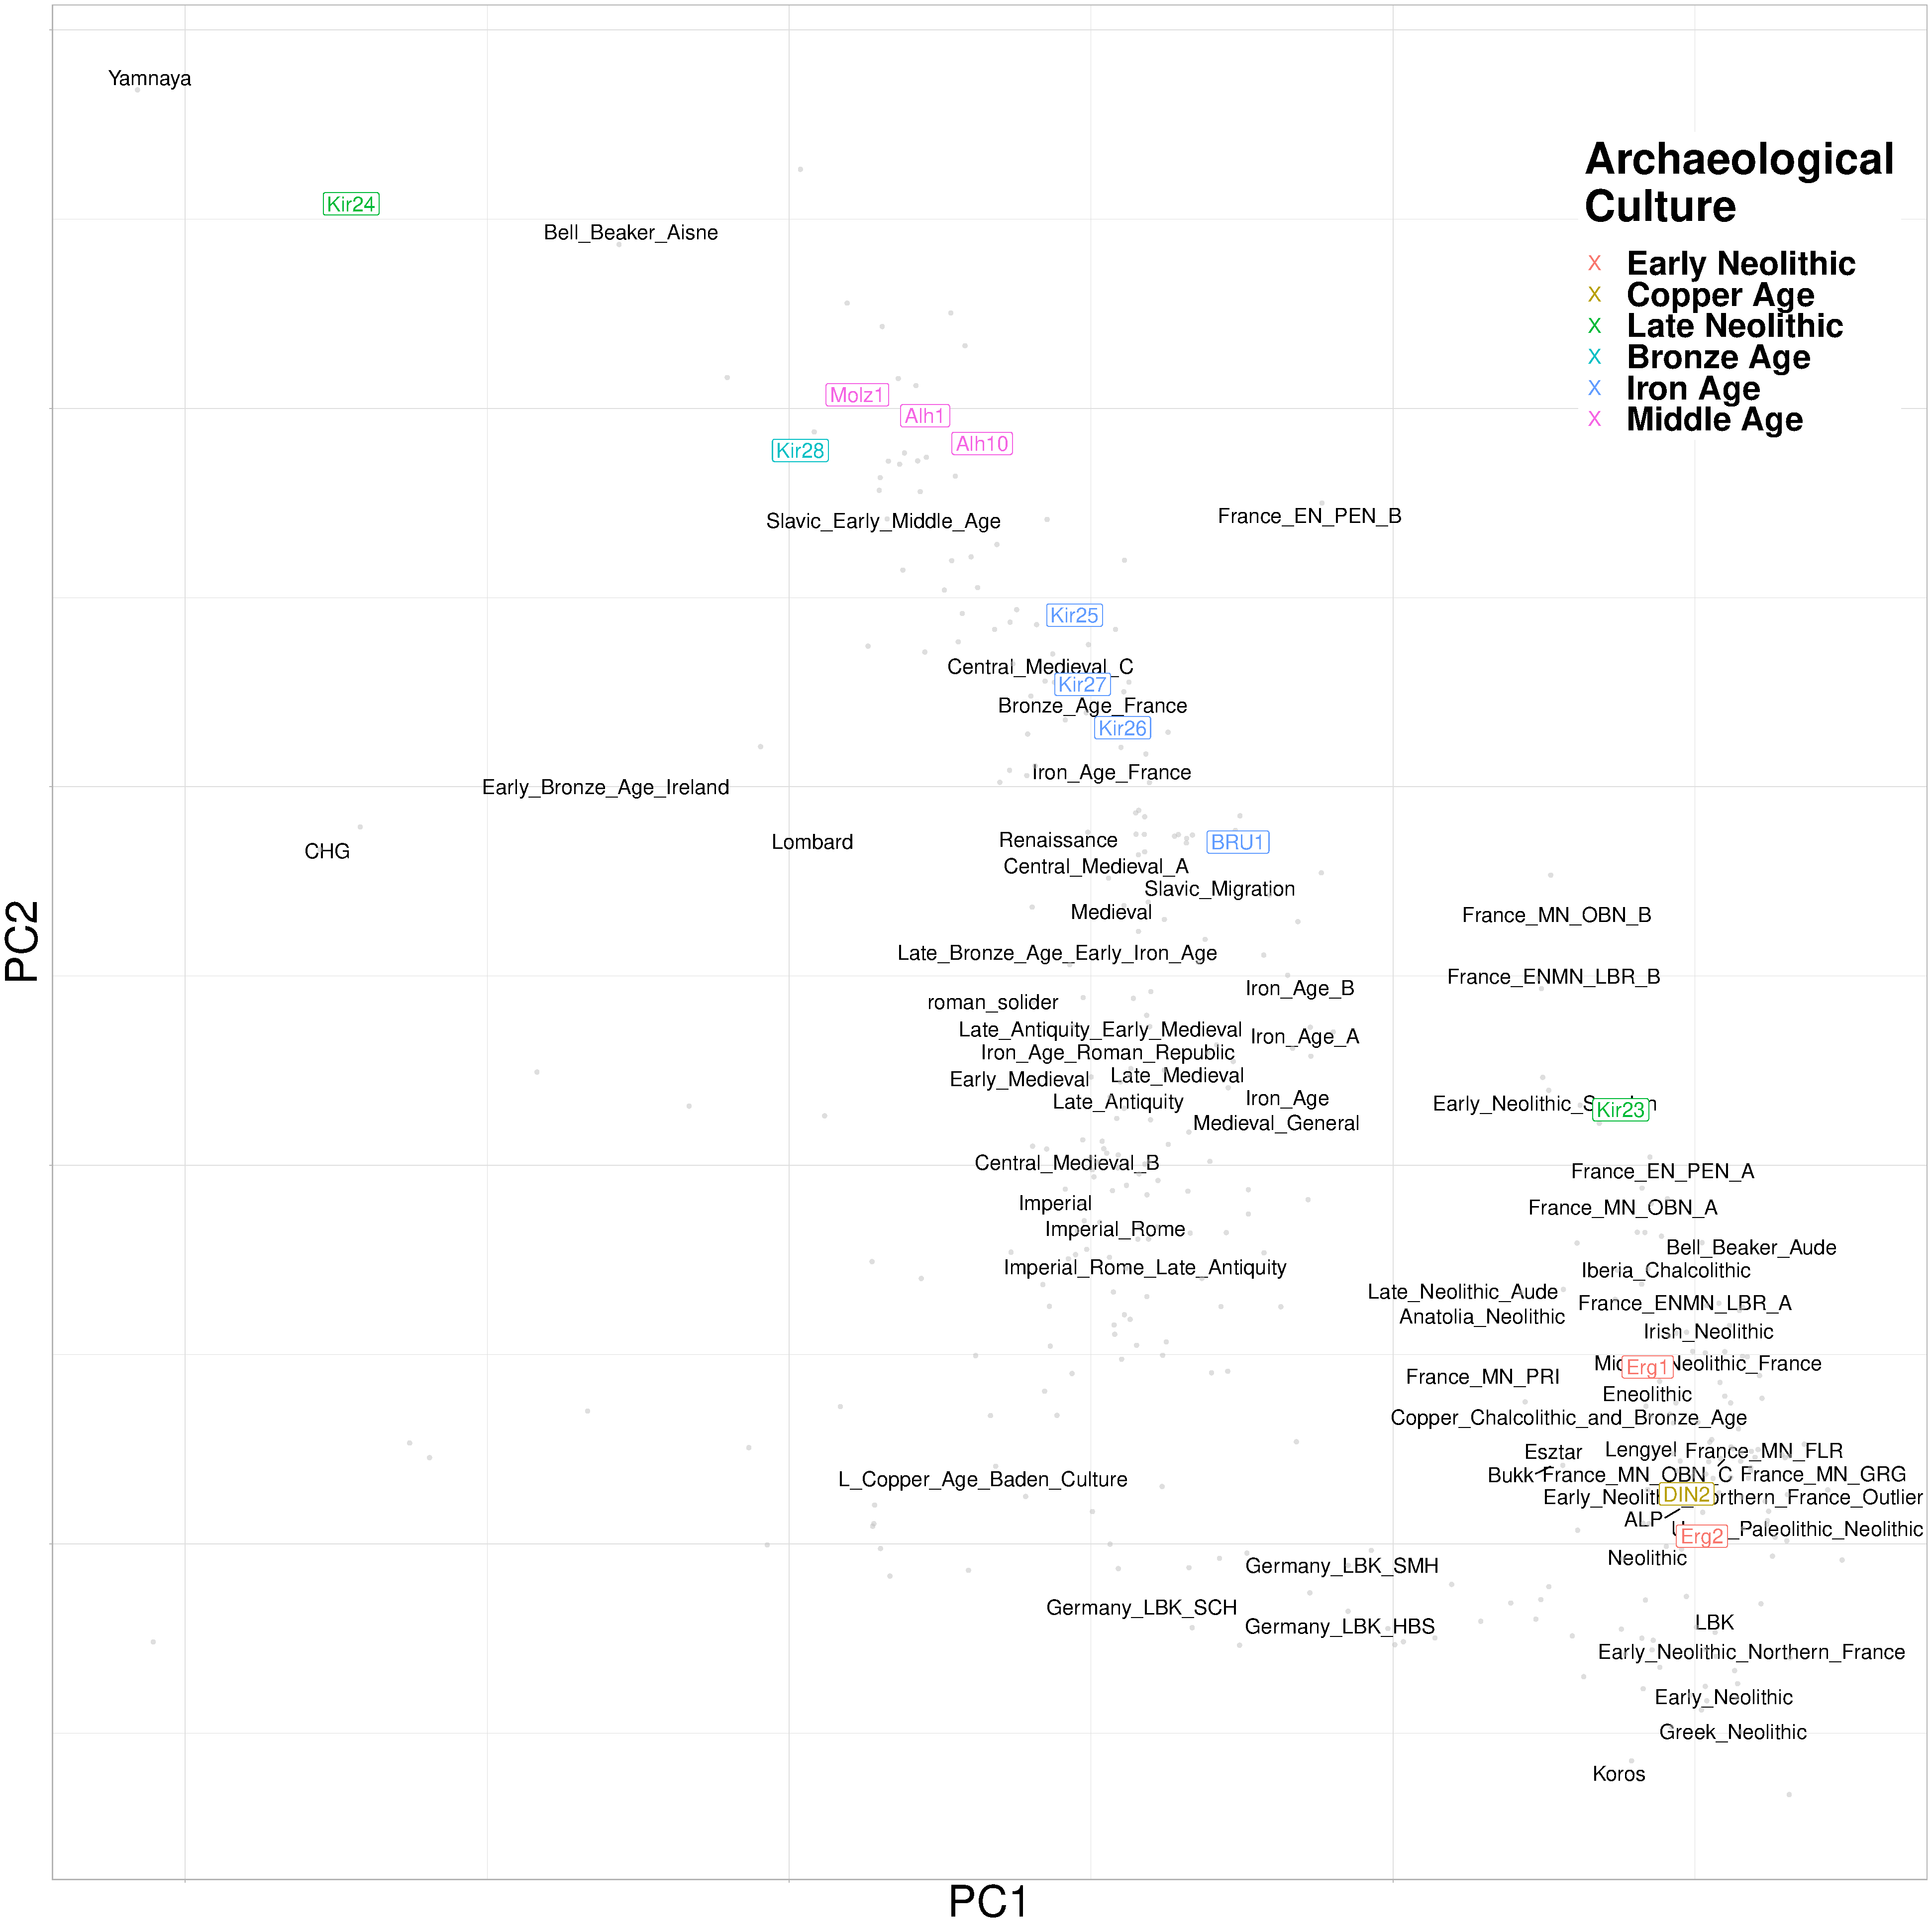
\includegraphics[width=1.0\textwidth]{../images/appendix/plink_withHG_PCA.pdf}
    \caption{Principle component analysis of genotype matrix using plink2. Grey points indicate principle component coordiantes for each sample. Black text indicated mean principle component coordinates for all individuals within that group. Coloured labels represent newly sequenced ancient samples. }
    \label{fig:plink_PCA_HG}
\end{figure}

\begin{figure}[htp]
    \centering
    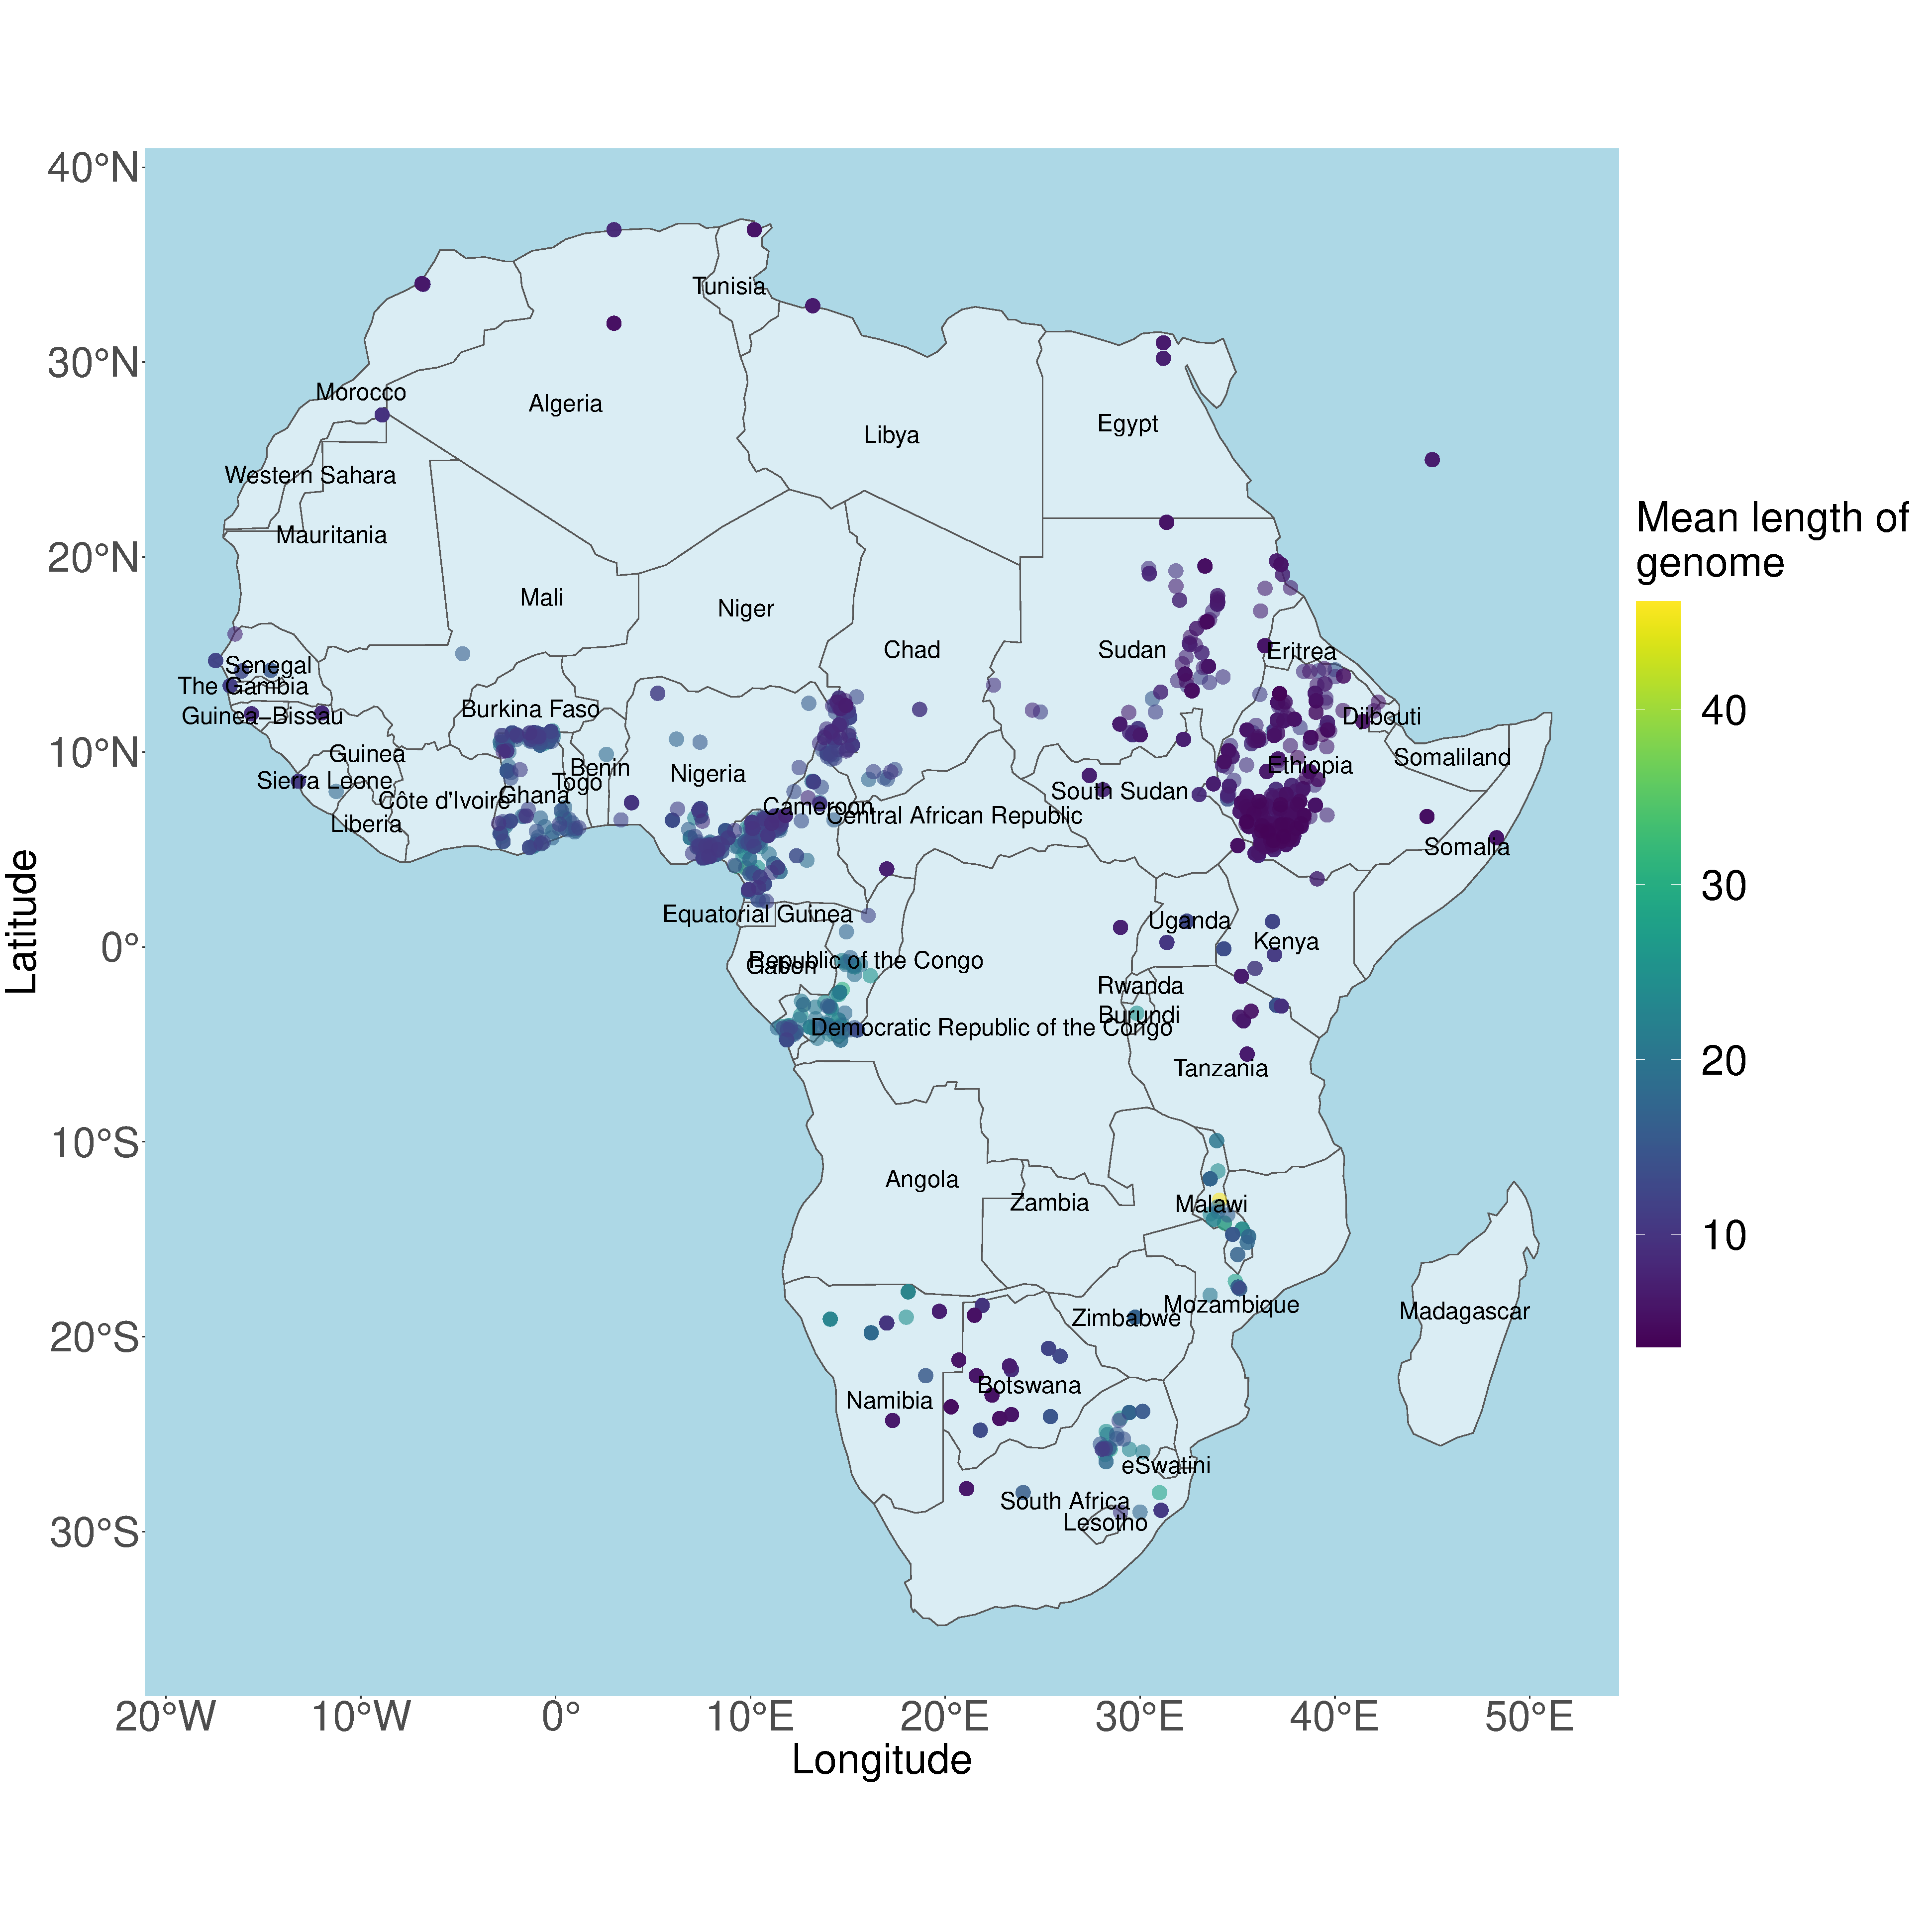
\includegraphics[width=1.0\textwidth]{../images/appendix/haplotype_map_Brazil.pdf}
    \caption{Map of haplotype donation to U.K. Biobank individuals born in Brazil. Each point represents one Human Origins population, coloured according to the summed amount of chunklengths that population donates to all U.K. Biobank individuals born in Brazil.}
    \label{fig:haplotype_map_Brazil}
\end{figure}

\begin{figure}[htp]
    \centering
    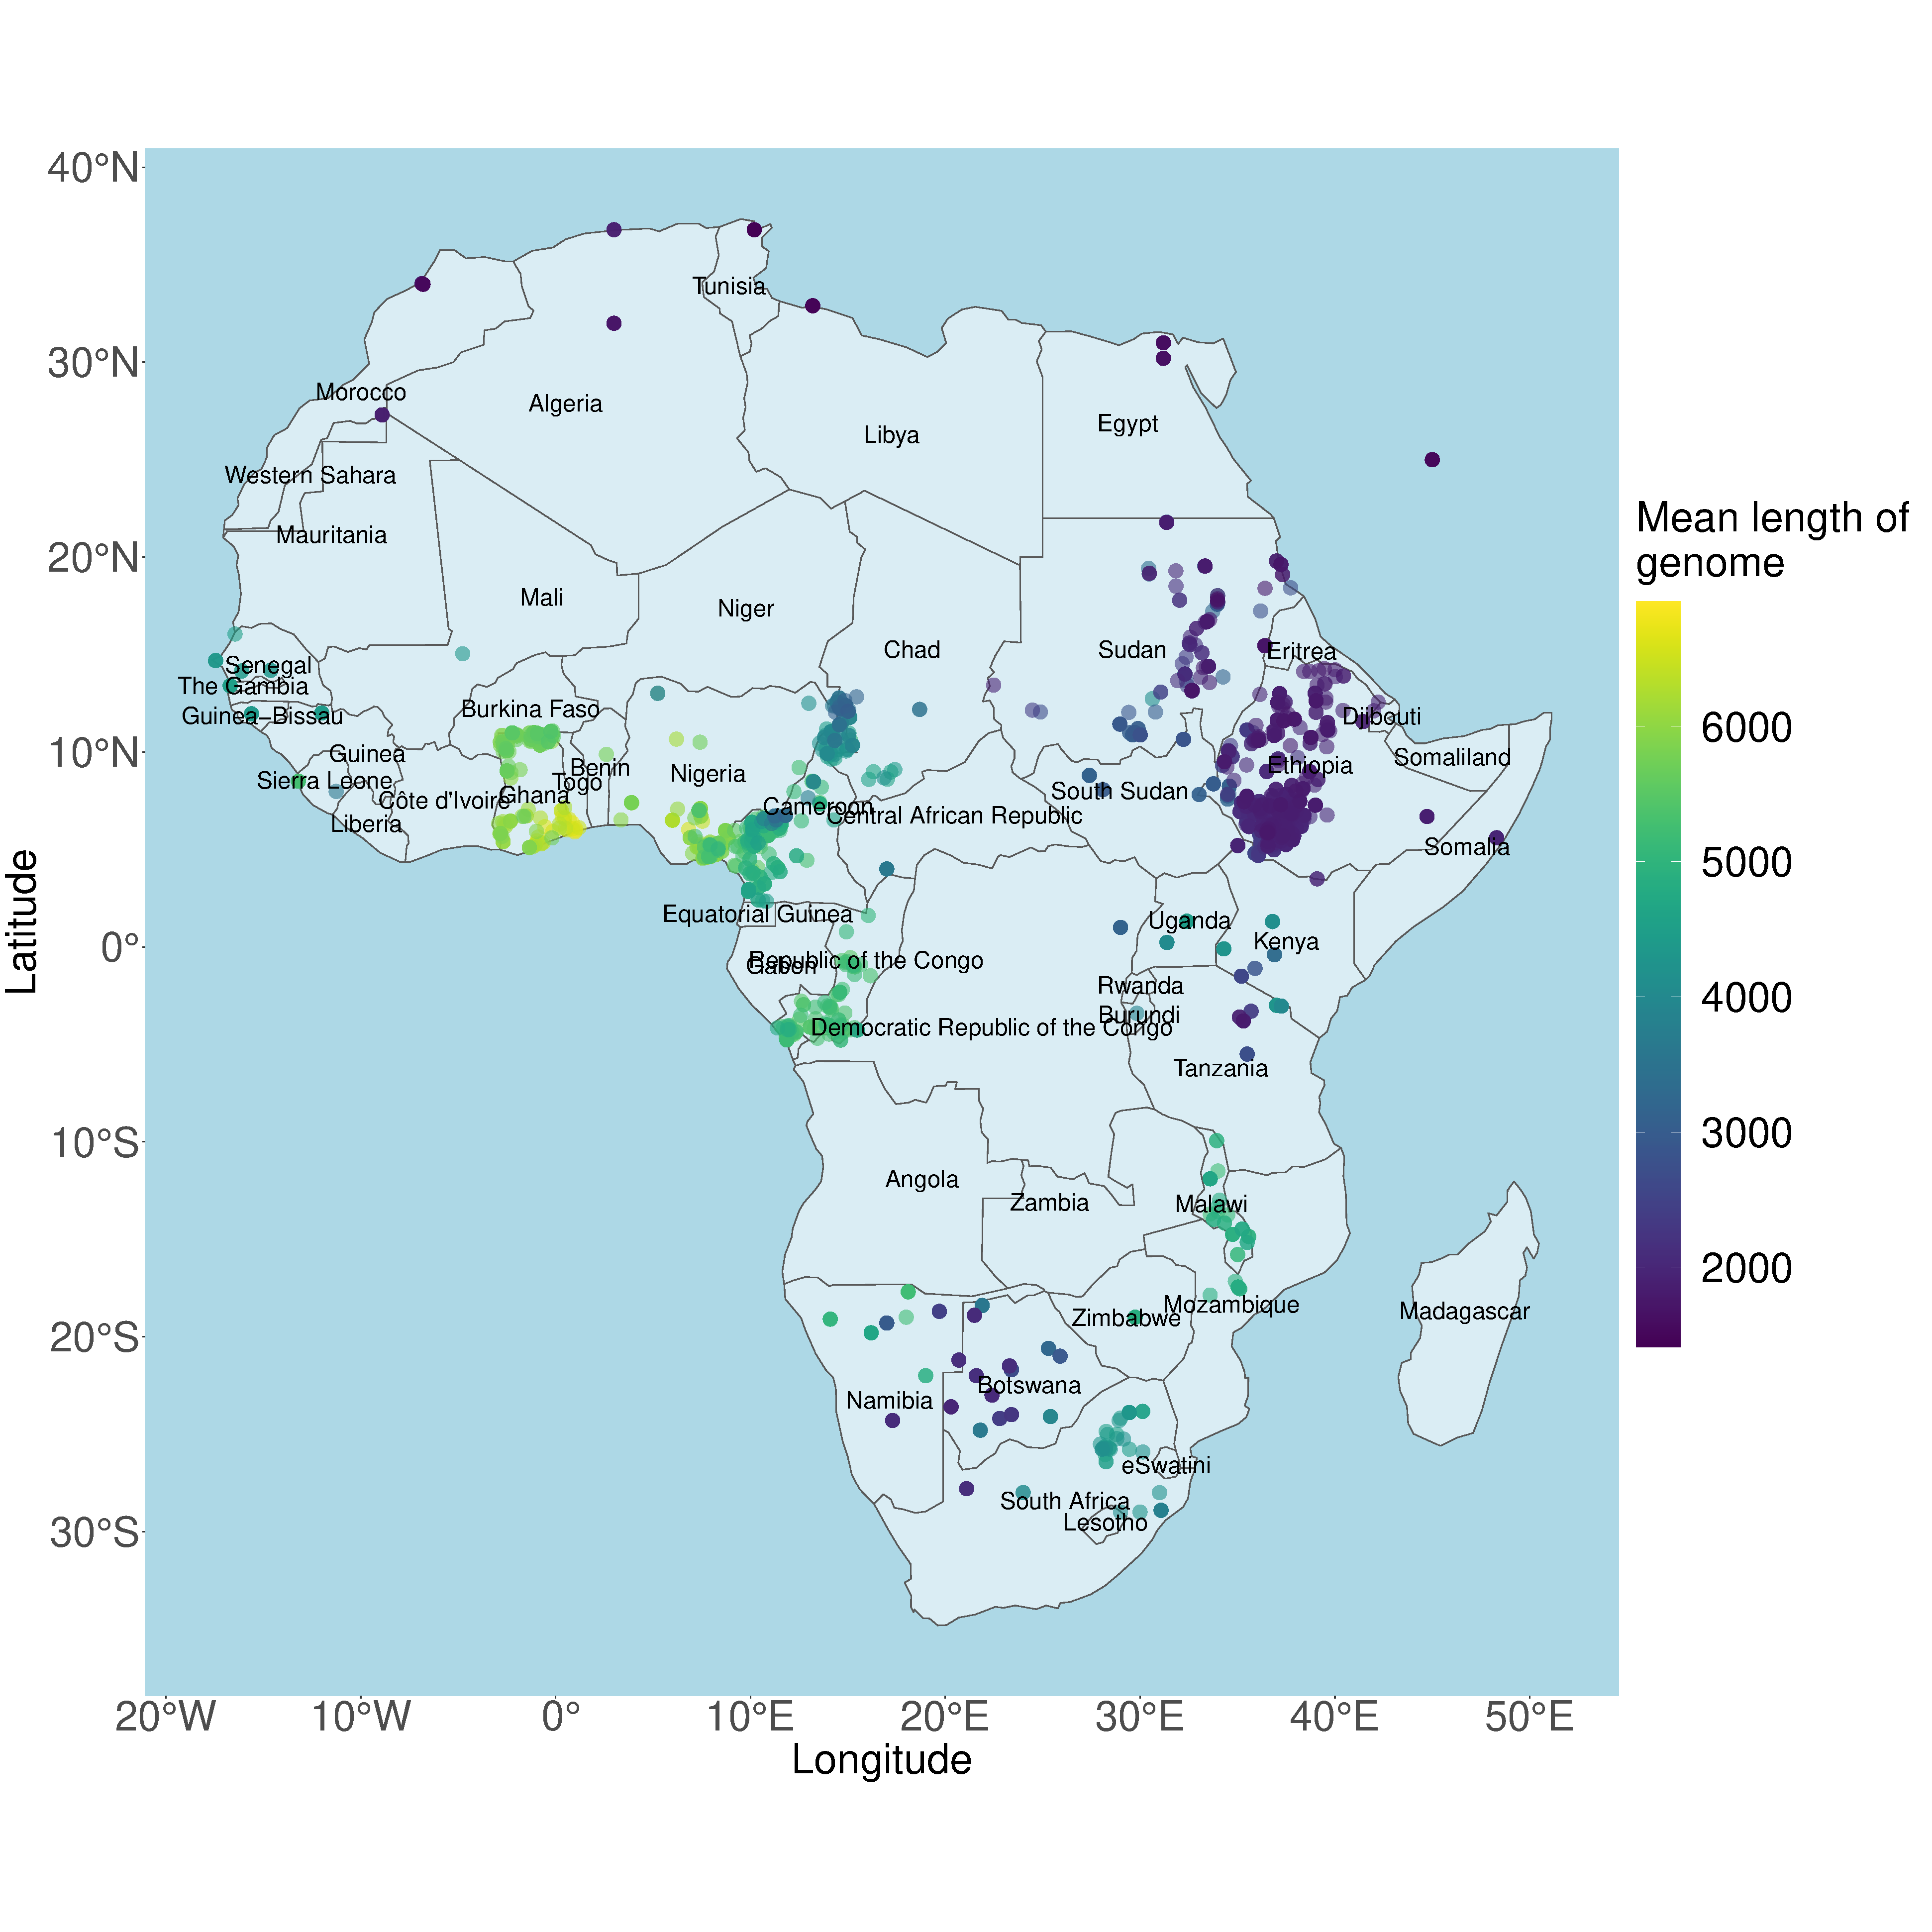
\includegraphics[width=1.0\textwidth]{../images/appendix/haplotype_map_Caribbean.pdf}
    \caption{PrMap of haplotype donation to U.K. Biobank individuals born in the Caribbean. Each point represents one Human Origins population, coloured according to the summed amount of chunklengths that population donates to all U.K. Biobank individuals born in the Caribbean.}
    \label{fig:haplotype_map_Caribbean}
\end{figure}

\begin{figure}[htp]
    \centering
    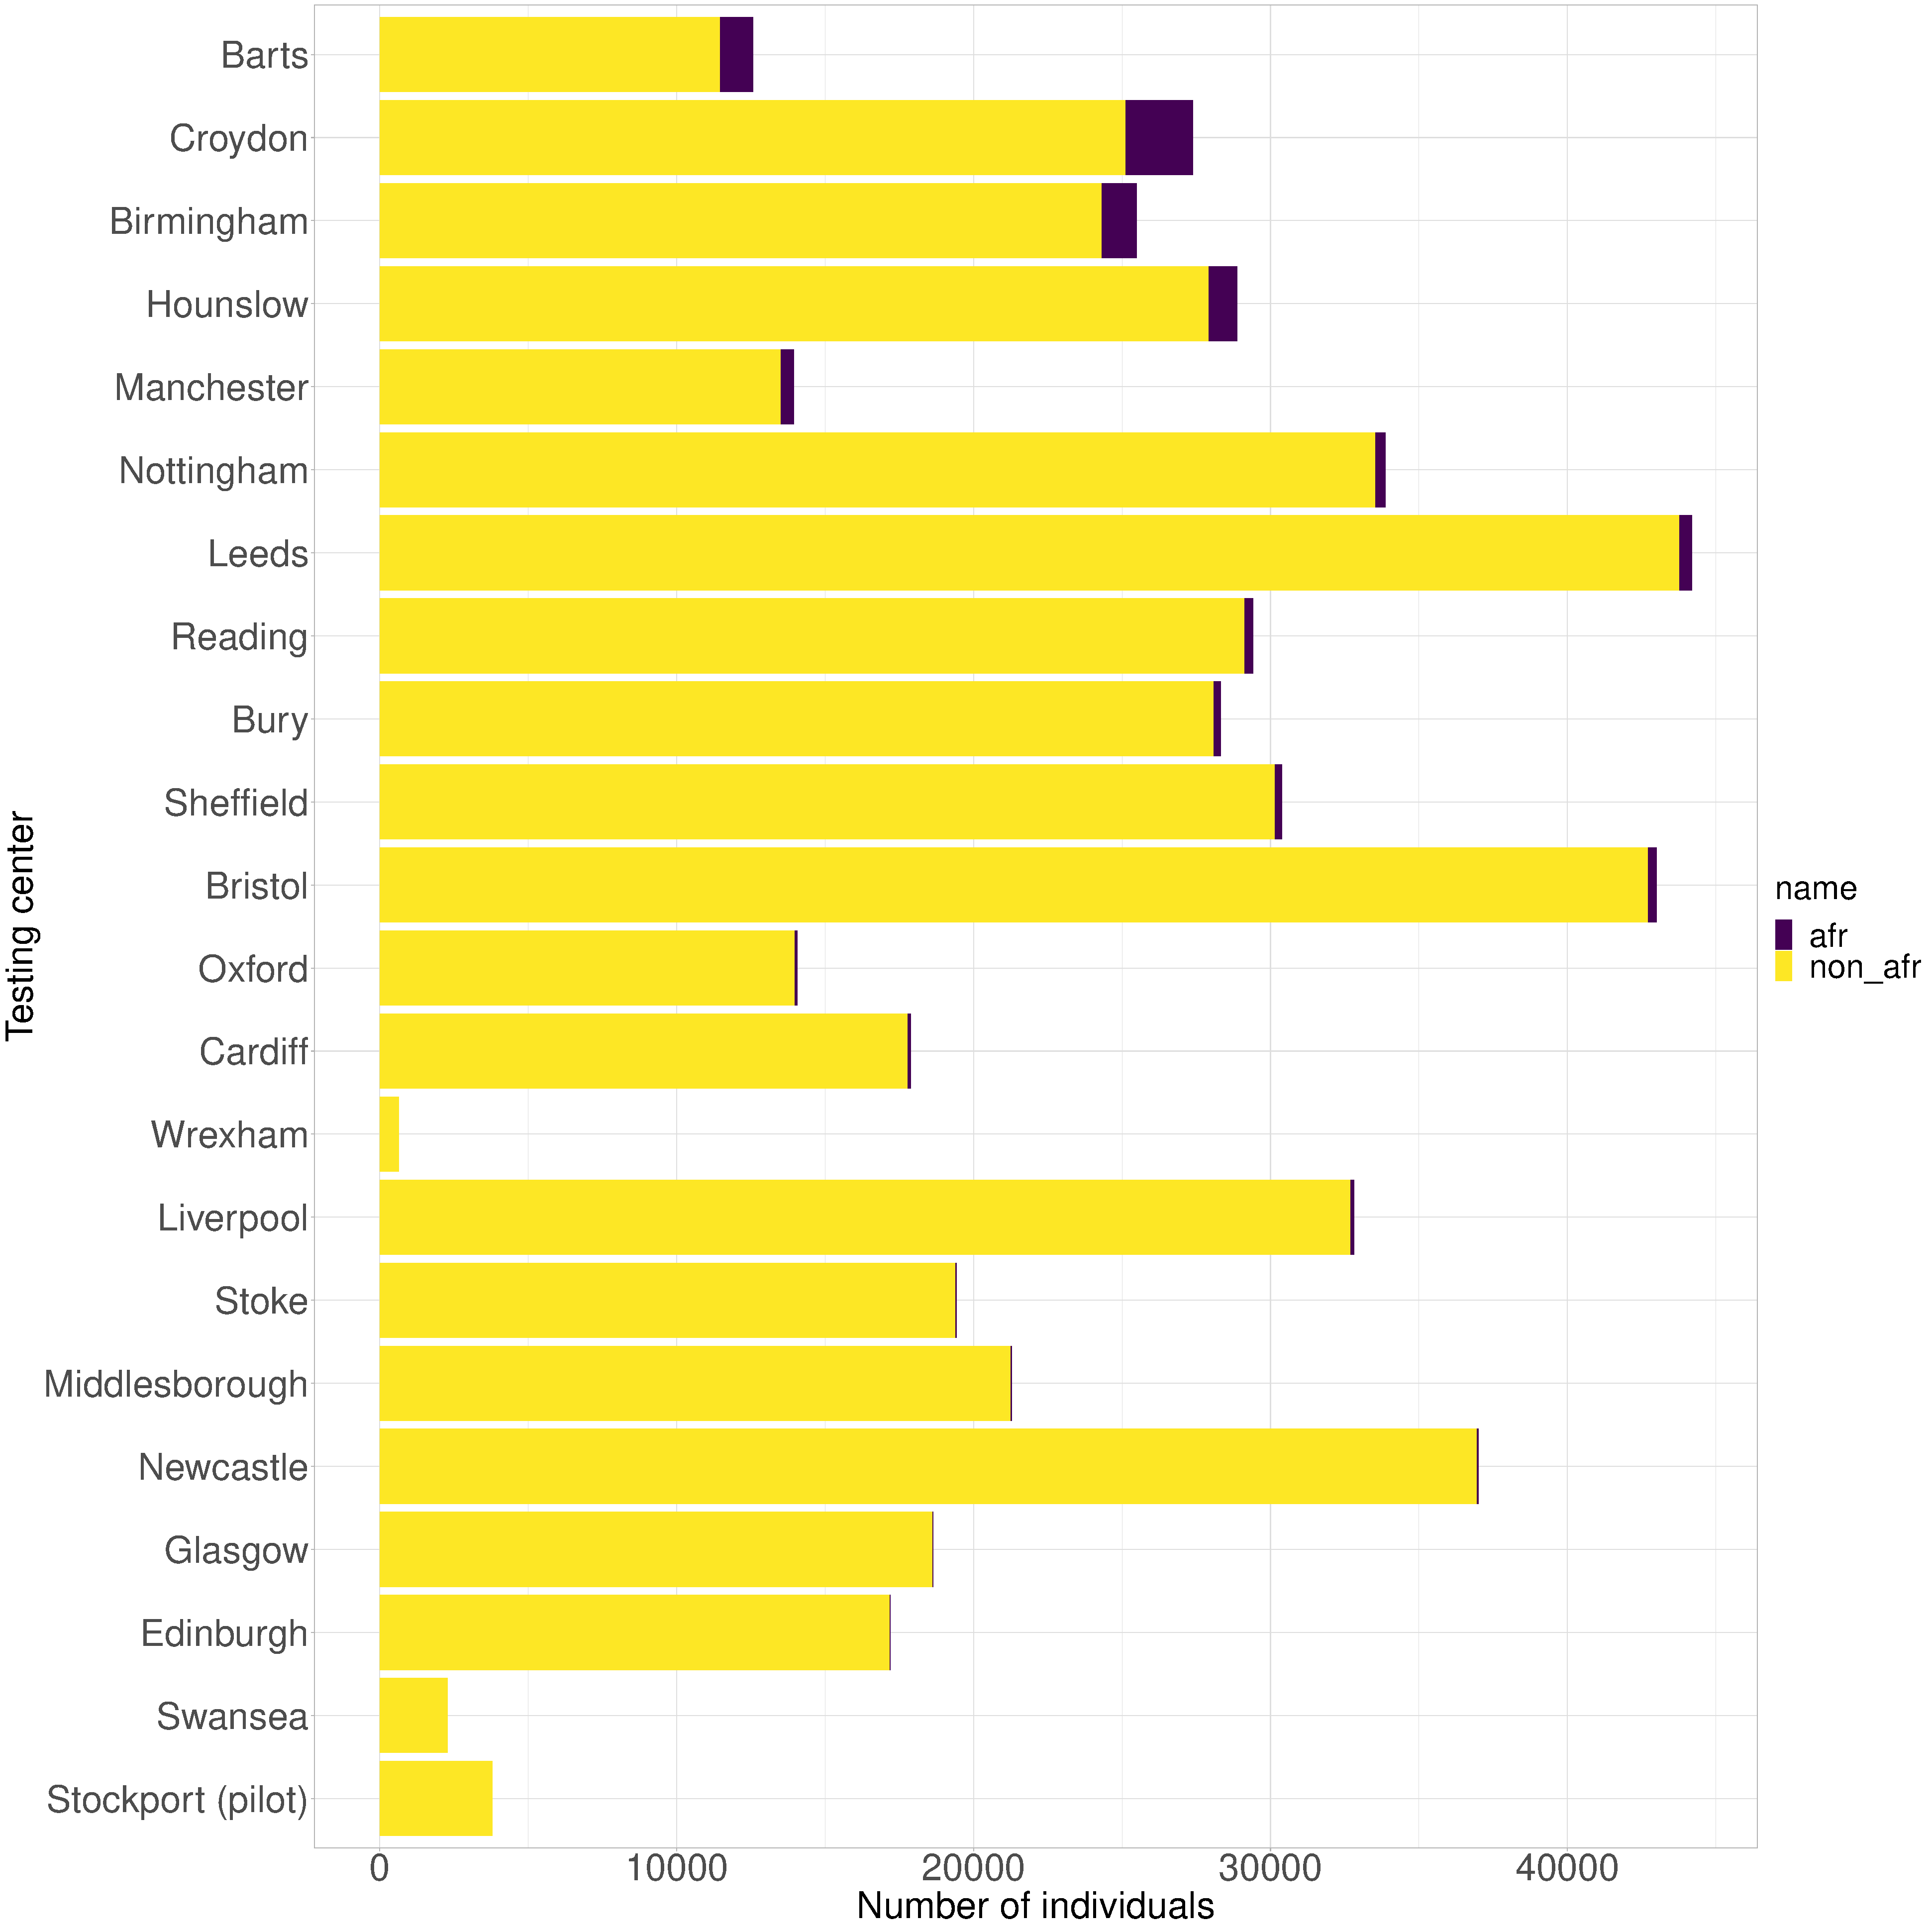
\includegraphics[width=1.0\textwidth]{../images/appendix/testing_centre_afr_prop.pdf}
    \caption{Number of total individuals and proportion of total individuals who have at least 50\% African ancestry by different testing centers. Centers ordered by proportion of individuals who have at least 50\% African ancestry.}
    \label{fig:haplotype_map_Caribbean}
\end{figure}

